\documentclass[12pt]{article}
\usepackage[a4paper, total={6.6in, 9.4in}]{geometry}

\setlength{\parskip}{3pt}

\usepackage{amsmath}
\usepackage{amssymb}
\usepackage{bm}
\usepackage{graphicx}
\usepackage{siunitx}
\usepackage{authblk}
\usepackage{url}
\usepackage{appendix}
\usepackage{booktabs}
\usepackage[font=small]{caption}
\usepackage{subcaption}
\usepackage{verbatim}

\usepackage [english]{babel}
\usepackage [autostyle, english = american]{csquotes}
\MakeOuterQuote{"}

\bibliographystyle{ieeetr}

\begin{document}

\title{Multi-phase classification of liquid crystal textures using convolutional neural networks}
\author{\textit{Joshua Heaton}\\\textit{10133722}}
\affil{Department of Physics and Astronomy, The University of Manchester}
\affil{MPhys project report}
\affil{Project performed in collaboration with James Harbon\\Supervisor: Dr Ingo Dierking}
\date{\today}

\maketitle

\begin{abstract}
This project investigates the application of convolutional neural networks (CNNs) to the classification of liquid crystal phases from images of their textures. Three CNN classifier model types are tuned and trained on five individual phase group datasets. The complete dataset includes images of the cholesteric phase, as well as smectic A, C, I and F phases, all extracted from polarised microscopy videos of various liquid crystalline compound samples. Three binary classification tasks, each including two liquid crystal phases, provide the foundational demonstration of CNN model viability. The highest mean test set accuracies obtained are $98\pm2\%$, $99\pm1\%$, and $93\pm6\%$, for cholesteric and smectic, smectic A and C, and smectic I and F datasets respectively. More complex multi-phase datasets are also created and investigated, with a three-phase cholesteric, fluid smectic, and hexatic smectic set in addition to a set containing all five individual phases. The highest mean test set accuracies for these classification tasks are $85\pm2\%$ for the three-phase set, and $87\pm3\%$ for the five-phase set. These results confirm and expand upon the conclusions of the first semester of the project, further demonstrating the efficacy of CNNs in identifying experimentally-captured liquid crystal texture images. However, the full potential of the models in this task may not be realised without significant expansion of the dataset.
\end{abstract}

\pagenumbering{gobble}
\newpage
\tableofcontents

\pagenumbering{gobble}
\newpage
\pagenumbering{arabic}

\section{Introduction}
Machine learning (ML) is the term assigned to a wide range of computer algorithms that use data to automatically improve their performance on a specific task. These tasks can take various forms, including decision-making, pattern recognition, and prediction  \cite{Murphy12}. A sub-field of ML known as deep learning generally consists of applying large-scale multi-layer neural networks, a type of algorithm inspired by the structure of the brain, to tasks involving highly complex abstractions of data. Such intensive algorithms typically require vast quantities of data and powerful computational resources to be trained effectively, with the advantage that they do not require any manual feature extraction \cite{Goodfellow16}. With the recent explosion in availability of such data and sophisticated computing technology, deep learning has seen a surge in interest and application among several fields \cite{Shrestha19}. Computer vision is one such field that has been impacted greatly. Convolutional neural networks (CNNs), a type of neural network suited particularly well to grid-based data, have proven extremely successful in the tasks of image classification, segmentation, and object detection \cite{Voulodimos18}.

There are many thousands of documented liquid crystal (LC) compounds, with each displaying a certain sequence of identifiable phases between that of a liquid and solid \cite{Dierking03}. Commonly, polarised microscopy (PM) is used to capture images of the textures produced by LC phases for identification by eye \cite{Dierking03}. Literature on ML for LC phase classification is sparse, with most studies focusing on the extraction of physical properties of LCs using simulated texture data \cite{Sigaki20, Sigaki19, Minor20, Walters19}, or other means \cite{Florin07, Butnariu13, Doi19, Inokuchi20}. Of most relevance is the work by Sigaki et al., in which they utilise CNNs to classify simulated isotropic and nematic phases to high accuracy \cite{Sigaki20}.

In this project, we prepare a novel dataset of LC texture images captured by PM, spanning multiple phases of all orders. Subsequently, we apply CNN classifier models to various phase groupings, probing the limits of attainable model accuracy. The work expands on and consolidates that of the first semester report \cite{Heaton20}, in which we demonstrated the viability of CNNs in some simple LC phase classification tasks. This report will provide a brief overview of LC phases, supervised ML, and neural networks. Further detail on each of these topics can be found in the first semester report \cite{Heaton20}. Details of the training methods and models used will then be provided, followed by a presentation of the results when they are applied to each of the prepared datasets. Summary conclusions and the limitations of the study will then be discussed.

\section{Background principles}
\subsection{Liquid crystals}
Liquid crystal phases are characterised by the positional and orientational order of the molecular arrangement. In general, the phase of lyotropic LCs depends on the concentration of the sample in a solvent whilst thermotropic LCs, used in this project, become more ordered with decreasing temperature \cite{Dierking03}. The order and overall structure of the LC phase determines its optical properties, in particular its birefringence. This enables images of the textures of a liquid crystal to be obtained by polarised microscopy, in which the sample is placed between two perpendicularly aligned polarisers. Polarised light incident on the set-up is altered depending on the current phase of the LC sample, producing characteristic features in the resulting image \cite{Dierking03}.

At sufficiently high temperatures, thermotropic LCs take the form of a fully anisotropic liquid with no structural order and hence no birefringence, resulting in completely dark PM textures. Upon cooling, they will display at least one higher ordered phase before reaching the fully crystalline stage. Of lowest order, just orientational, is the nematic (N) phase, where the molecules are aligned along a particular axis called the director and are still free to move around as in a liquid. Compounds with chiral molecules may instead display the cholesteric (Ch) phase, which is the same as the nematic phase except with helical variation of the director. Layered positional order is introduced in the smectic phase (Sm), which is divided into three distinct phase groupings. The orientation of the director further categorises these groupings. The fluid smectic (FSm) phases have no positional order within molecular layers. The orientation of the director with respect to the layer planes determines whether the phase is smectic A (SmA), in which it is perpendicular, or C (SmC) otherwise. The smectic B (SmB), I (SmI), and F (SmF) phases are placed into the hexatic smectic (HSm) group, with short-range hexagonal structures generating positional order within the layers. The soft crystal phases differ in that the layers show long-range positional order \cite{Dierking03}.

This project uses CNNs to classify PM textures from thermotropic chiral LC compounds, including the phases Ch, SmA, SmC, SmI, and SmF. Figure \ref{textures} gives an example texture image from each of these phases.
\begin{figure}[!h]
\centering
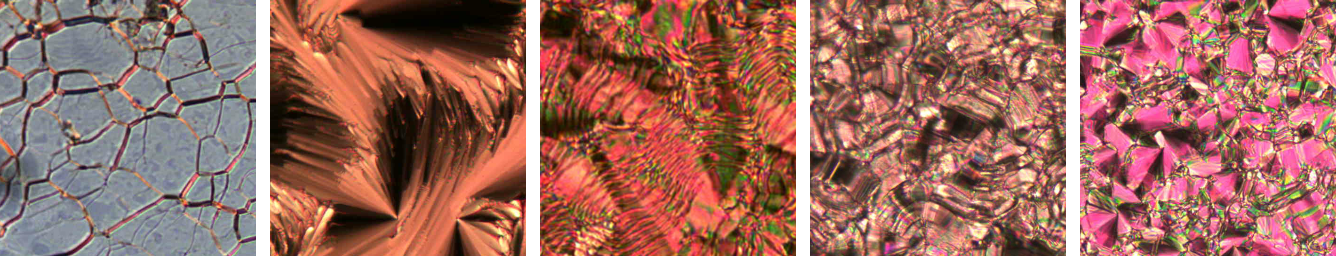
\includegraphics[width=\textwidth]{images/textures.png}
\caption{Samples from our complete LC phase texture dataset, from left to right: Ch, SmA, SmC, SmI, and SmF.}
\label{textures}
\end{figure}  

\subsection{Supervised machine learning}
Machine learning algorithms can in general be categorised as supervised, unsupervised, or reinforcement learning \cite{Murphy12}. The ML implementations of this project are purely supervised learning algorithms. In this case, the ML model is defined as a function, parametrised by learned values $\bm{\theta}$, that maps an input data sample $\bm{x}$ containing various features to an output predicted label $\hat{\bm{y}}$ \cite{Murphy12},
\begin{equation}
\hat{\bm{y}}=f(\bm{x};\bm{\theta}). \label{supmodel} 
\end{equation}
$\hat{\bm{y}}$ can take various forms depending on the specific task, for example regression, in which the model attempts to predict a continuous value given the input data, or classification, in which it predicts a category that the input data sample belongs to \cite{Murphy12}. A supervised model attempts to learn appropriate $\bm{\theta}$ values for the mapping using a set of training data, consisting of pairs, $i$, of input examples and their corresponding true labels, $\lbrace\bm{x}^{(i)},\bm{y}^{(i)}\rbrace$. The model takes sample $\bm{x}^{(i)}$ and produces an output label prediction $\hat{\bm{y}}^{(i)}$ according to Equation \ref{supmodel} \cite{Murphy12}. A chosen cost function $J(\bm{y},\hat{\bm{y}};\bm{\theta})$ is then evaluated, which generally provides a measure of the divergence of the model outputs from the true labels. The parameters are then updated with a particular optimisation algorithm in order to minimise the cost. Successful training as such results in a model that is effective in producing accurate predictions for new unseen data samples \cite{Murphy12, Goodfellow16}. Fixed parameters that define the precise form of $f$, as well as training configurations, are known as hyperparameters \cite{Murphy12, Goodfellow16}.

When deciding on the form of a supervised model, of great importance is its capacity, which can be thought of as the size of the model. A low capacity model with few trainable parameters may not extract or infer enough features from the training data to form accurate predictions, a problem called underfitting. On the other hand, too high a capacity will cause the model to learn many meaningless features from the training data and it may not perform well when inferring on new unseen examples. This is referred to as overfitting. The model's hyperparameters must, therefore, be properly tuned to ensure it does not overfit or underfit. In addition to limiting model capacity, regularisation techniques can be applied to help prevent overfitting and improve generalisation \cite{Murphy12, Goodfellow16}.

Measurement of a supervised model's performance is critical in determining how well it will generalise to new unseen data, often done by evaluating a metric on a dataset of samples. For classification tasks a common metric is the percentage of samples that the model assigned the correct class label \cite{Murphy12}. The training dataset can be split into three subsets: training, validation, and test. The training set contains the data samples used to update the trainable parameters of the model. The validation set is used to tune the hyperparameters of the model. Evaluation of a trained model on the training and validation sets can reveal if the model has underfitted or overfitted. In the former case a low performance on both sets will be observed, whereas for the latter a high performance on the training set and low on the validation set will occur \cite{Murphy12, Goodfellow16}. Hyperparameters can then be adjusted accordingly before retraining the model. After a satisfactory model configuration and validation performance are reached, it is evaluated on the as-of-yet unseen test set to give an indication of the model's generalisation error \cite{Murphy12, Goodfellow16}.

\subsection{Neural networks}
\subsubsection{Layers}
Neural networks are a type of ML algorithm that pass input data through a series of layers, each containing a number of units. Every unit of a layer is connected in a particular way to the units of the previous layer. Units can take various forms including ones with or without trainable parameters, and specific layers are engineered so as to identify, manipulate, and propagate data features from the input to the output of the network \cite{Haykin98}. In a fully-connected, or dense, layer the input to each unit is the outputs of all units of the previous layer. The inputs are multiplied by the unit's learned weight parameters and summed together with a learned bias parameter to calculate the unit's output \cite{Goodfellow16, Haykin98}. An activation function can then be applied to the output of each unit of the layer to introduce non-linearity to the network. Such non-linearities are essential in allowing a neural network to act as a universal function approximator, enabling it to perform highly complex inference on input data \cite{Hornik89}. A dense layer can hence be represented in matrix form as
\begin{equation}
\bm{O}=A(\bm{W}\bm{I}+\bm{B}), \label{dense}
\end{equation}
where $\bm{O}$ is the vector containing the outputs for the layer, $\bm{W}$ is the matrix of layer weights, $\bm{I}$ is the vector of layer inputs, $\bm{B}$ is the vector of bias parameters, and $A$ is the activation function applied element-wise \cite{Goodfellow16, Haykin98}.

Convolutional layers take grid-based input data such as two-dimensional images, and convolve it with a kernel of trainable parameters. The kernel has a width and height smaller than that of the input. The kernel is moved iteratively over the input, with the distance moved each iteration known as the stride of the convolution \cite{Aghdam17}. At each step the kernel's parameters are multiplied with aligned input values, with the results summed together to produce the final output value. An activation function can be applied to this output value. The complete layer output is formed as a grid containing the ordered output values from the convolution. The size of the output grid depends on the dimensions of the kernel and the stride of the convolution, as these together determine the number of convolution steps in each direction \cite{Aghdam17}. The input and output of the layer can have a third dimension, for example with the three colour channels of an RGB image. In this case, the kernel will have a different set of parameters for each channel. The number of channels can be increased from input to output by stacking the results from multiple kernels \cite{Aghdam17}. A convolutional layer's padding refers to the behaviour of the kernel at the edges of the input. When the kernel is confined completely within the input space it is called valid padding. Same padding is when the kernel extends beyond the input space such that each value is visited by the kernel the same number of times, with kernel values outside the space multiplied by zero. For a stride of one in both directions, same padding will result in an output with the same shape as the input, and valid padding will result in dimensionality reduction \cite{Goodfellow16, Aghdam17}. An example of a convolution operation is detailed in Figure \ref{convop}.
\begin{figure}[!h]
\centering
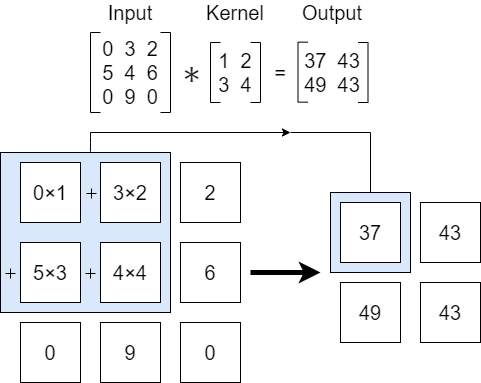
\includegraphics[width=0.5\textwidth]{images/convolution.png}
\caption{Adapted from \cite{Goodfellow16}. An example convolution operation with one channel. The $3\times3$ input is convolved, denoted by $\ast$, with a $2\times2$ kernel with stride $1\times1$ and valid padding, to produce a $2\times2$ output matrix.}
\label{convop}
\end{figure}

The main advantage of convolutional layers over dense layers is the greatly reduced computational and memory cost, since they require far fewer parameters. The kernel parameters are shared over the entire input, which can also improve regularisation. Each kernel can be thought of as learning to extract a particular feature from the input to be passed on to the next layer, such as edges of objects in an image \cite{Goodfellow16}.

Pooling layers are often used after convolutional layers to reduce the dimensions of the network \cite{Goodfellow16}. They work analogously to convolutional layers, however, the kernel has no trainable parameters to convolve and instead performs a specific operation. This could be, for example, taking the maximum value from the aligned input values at each step, known as max pooling. Average pooling takes the arithmetic mean of the aligned input values \cite{Aghdam17}. For pooling layers the kernel size is instead known as the pool size, and the pooling operation is applied to each input channel individually. Global pooling refers to the case in which the pool size is equal to the input size, which results in a vector output with one value for each of the input channels \cite{Aghdam17}. Pooling layers are utilised to reduce the overall size and computational cost of the network whilst providing it with some invariance to translations of the input \cite{Goodfellow16, Aghdam17}.

A common choice of activation function for dense and convolutional layers is the rectified linear unit (ReLU), defined for unit output $z$ as
\begin{equation}
A(z)=\mathrm{max}(0, z), \label{relu}
\end{equation}
which partially models the behaviour of neurons in the brain \cite{Glorot11}. It has the advantage of introducing non-linearity without the potential for vanishing or exploding gradients when training the network \cite{Goodfellow16, Glorot11}. For classifier neural networks, the final output layer is a dense layer with a number of units equal to the number of classes. The softmax activation function is applied, which converts the output of each unit into a probability that the input sample belongs to the unit's corresponding class \cite{Goodfellow16}. For output unit $i$, this is defined as
\begin{equation}
\sigma(\bm{z})_i=\frac{e^{z_i}}{\sum_{j=1}^Ne^{z_j}}, \label{softmax}
\end{equation}
where $N$ is the total number of classes. The final output of the network is generally taken as the class with the greatest assigned probability \cite{Goodfellow16}.

\subsubsection{Training}
Before training begins, a neural network's trainable parameters are randomly initialised from a particular distribution such as a normal distribution \cite{Goodfellow16}. A training step is performed by first selecting a "minibatch" containing a set number, called the batch size, of random samples from the training set of data. The samples are passed through the network and a loss function is evaluated for each output \cite{Goodfellow16}. For classifier models, a widely used loss function, derived from the Kullback–Leibler divergence and maximum likelihood estimation, is the categorical cross-entropy, defined as
\begin{equation}
L(p)=-\mathrm{log}p
\end{equation}
where $p$ is the model's output probability that the sample belongs to the true labelled class \cite{Kline05}. The cost function is then calculated as the average of the loss for all samples in the minibatch \cite{Goodfellow16}. An algorithm called backpropagation is then applied to calculate the gradient of the cost function with respect to the trainable parameters, $\bm{g}=\bm{\nabla}_{\theta}J(\bm{y},\hat{\bm{y}};\bm{\theta})$. Backpropagation, in summary, applies the chain rule of differentiation sequentially from the final network layer going backwards to the input layer, extracting the gradients at each unit output \cite{Goodfellow16, Amari93}. A chosen optimisation algorithm is then applied to update the parameters, with a simple example being stochastic gradient descent \cite{Goodfellow16}. In this case, the parameters are updated against the gradient as
\begin{equation}
\bm{\theta}\leftarrow\bm{\theta}-\alpha\bm{g},
\end{equation}
where $\alpha$ is a hyperparameter called the learning rate, which modulates how much the parameters are adjusted with each step \cite{Amari93}. This act of descending the cost function aims to reduce the loss when the model is evaluated on future samples, and in doing so improve its accuracy \cite{Goodfellow16}. Minibatches are sampled without replacement until the entire training set has been observed by the model, completing an epoch of training \cite{Goodfellow16}.

\subsubsection{Regularisation methods}
There are numerous methods of regularising neural networks in order to negate overfitting \cite{Goodfellow16}. Here the details are provided for methods utilised in this project.

Dataset augmentation aims to effectively increase the overall number of samples in the training set by performing transformations on the samples when they are selected for a minibatch, with the result taking the same label as the base sample. In the case of image data, alterations can be applied randomly and can include flipping the image, rotations, translations, and magnification within certain ranges. When used appropriately, augmentations are a powerful and simple way to improve model generalisation \cite{Goodfellow16}.

Another simple yet highly effective regularisation method is early stopping. During training the model's performance on the validation set, usually simply the cost evaluated on the entire set, is recorded after every training epoch. Training stops if the cost has not decreased by more than a tolerance value after a certain number of epochs, defined by the patience hyperparameter. This helps greatly with regularisation because the model can overfit the training set if trained for too many epochs \cite{Goodfellow16, Bishop95}.

Dropout is a regularisation technique in which unit outputs in a layer are multiplied by zero with a set probability, called the dropout rate, with random units selected each training update step. This can be viewed as training multiple sub-models with shared parameters, and it has the effect of reducing the neural network's sensitivity to noise \cite{Srivastava2014}.

For a layer with batch normalisation, after calculating the layer output values for each sample in a minibatch, the outputs are rescaled by subtracting the minibatch mean for each unit output and dividing by the standard deviation. The result for each unit is then rescaled linearly with extra learnable parameters. For output $z$ of a layer's unit this change is represented as
\begin{equation}
z\leftarrow\gamma\left(\frac{z-\mu}{\sigma}\right)+\beta, \label{batchnorm}
\end{equation}
where $\gamma$ and $\beta$ are the extra learnable parameters, $\mu$ is the mean and $\sigma$ is the standard deviation of the unit's output over the minibatch. For future computations on single samples, during training running averages of the means and standard deviations are recorded. Batch normalisation improves model stability whilst training and provides a regularising effect by introducing a form of noise \cite{Ioffe15}.

\section{Methodology}
\subsection{Data preparation}
All LC texture image data used has been obtained from PM videos of LCs, labelled by compound and temperature range. If not provided, the phases displayed in the videos are identified using project supervisor Ingo Dierking's co-authored papers on a homologous LC series \cite{Dierking94, Schacht95}. The software VLC Media Player \cite{VideoLan06} is used to extract image frames from the videos, and they are classified  according to the LC phase displayed at the point of extraction. The raw images have a resolution of $2048\times1088$. They are split into six smaller images of size $682\times544$ without compromising the features displayed by each image. The images are then cropped to square $544\times544$ before being scaled down to the model input size of $256\times256$ and converted to greyscale with pixel value range zero to one. This input size is selected based upon results of the first semester \cite{Heaton20}.

In construction of the training, validation, and test data sets, images of the same phase that also come from the same video are not divided between any of the three sets. This is to minimise potential data leakage, which is when samples in the training set are highly similar to samples in the validation or test sets, artificially inflating model accuracy on the validation or test set \cite{Kaufman12}.

The distribution of the complete dataset over all LC phases is presented in Figure \ref{datasetgraph}. 
\begin{figure}[!h]
\centering
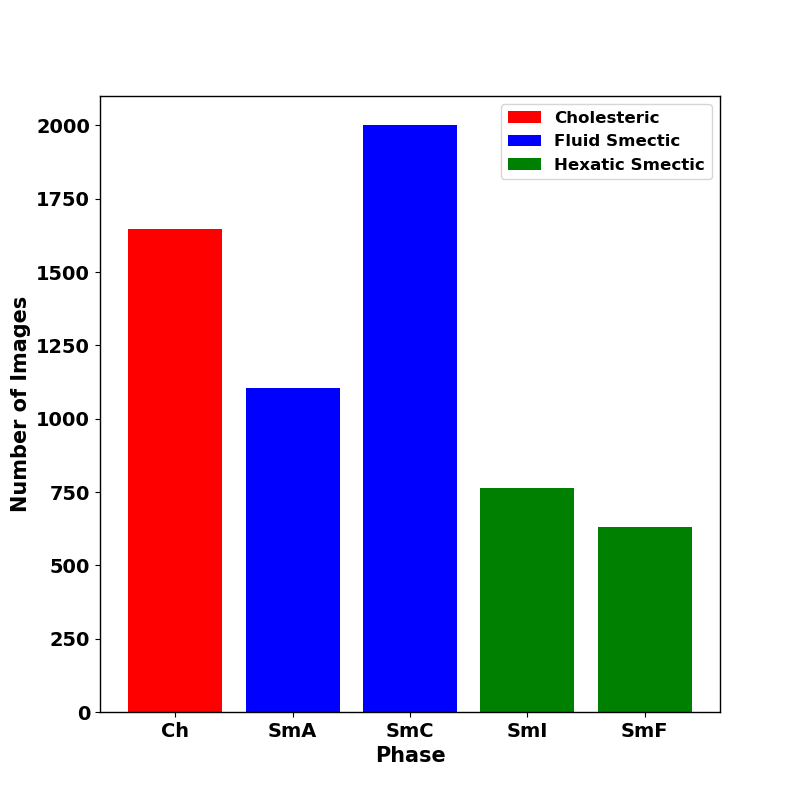
\includegraphics[width=4in]{images/Graphs/overalldataset.png}
\caption{The number of images in the complete dataset belonging to each phase, with a total of 6,978 images.}
\label{datasetgraph}
\end{figure}
From this we construct five individual model training datasets, split by video in an approximate ratio of 3:1:1 training to validation to test set image count. Videos are selected randomly from the training set to be moved into the validation and test sets until the target split ratio is approximately met. The five phase groupings includes three binary, or two-phase, sets and two multi-phase sets. The names of each dataset and the phases they include are summarised in Table \ref{datasets}, with the specific distributions of the data in each set presented in Appendix \ref{datdist}.
\begin{table}[!htb]
\begin{center}
\caption{The LC phases contained in each dataset.}
\begin{tabular}{l|c|c|c|c|c}
\toprule
\textbf{Dataset} & ChSm & SmAC & SmIF & ChSm2 & ChSm4\\
\midrule
\textbf{Phases} & Ch, Sm & SmA, SmC & SmI, SmF & Ch, FSm, HSm & Ch, SmA, SmC, SmI, SmF\\
\bottomrule
\omit
\label{datasets}
\end{tabular}
\end{center}
\end{table}

\subsection{CNN Models}
In this project we use three different types of CNN architectures, with each built from dense, convolutional, and pooling layers. All convolutional layers use a stride of $1\times1$, same padding, and ReLU activation, and all dense and convolutional layers have batch normalisation. A standard convolutional layer has kernel size $3\times3$, and a standard pooling layer refers to a max pooling layer with pool size and stride of $2\times2$ and same padding.

\subsubsection{Sequential}
The simplest and lowest capacity models used are Sequential CNNs. They consist of a series of standard convolutional layers, each followed by a standard pooling layer. The number of channels is doubled with each successive convolutional layer. The final convolutional layer in the network is followed instead by global average pooling, which is proceeded by two dense layers, first with a number of units equal to the output of the average pooling, and second with half this. Both dense layers have ReLU activation and dropout rate 0.5. The final layer is the dense classification output with a number of units equal to the number of classes and a softmax activation. Figure \ref{seqarch} displays a diagram of a Sequential model with three convolutional layers.
\begin{figure}[!h]
\centering
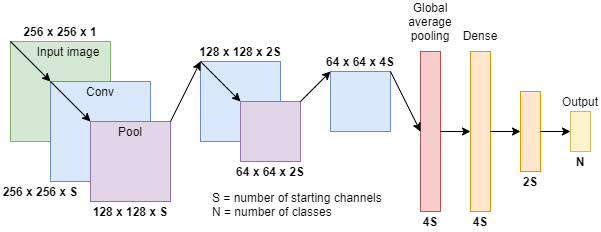
\includegraphics[width=0.9\textwidth]{images/sequential.png}
\caption{Schematic of a Sequential network with three convolutional layers. "Conv" refers to a standard convolutional layer and "Pool" to a standard pooling layer. Layer output shape is given in bold next to each layer.}
\label{seqarch}
\end{figure}

\subsubsection{Inception}
A set of models based on Google's Inception CNN architecture contain modules called Inception blocks, which have parallel convolutional layers with different kernel sizes sharing inputs and outputs \cite{Szegedy15}. The structure of an Inception block is detailed in Figure \ref{arch:inc}. Our downsized Inception networks begin with a convolutional layer with kernel size $7\times7$, followed sequentially by a standard pooling layer, a convolutional layer with kernel size $1\times1$, a standard convolutional layer, and a standard pooling layer. The output of this pooling layer is then fed into a series of one or more Inception blocks. The output of the final Inception block is followed sequentially by an average pooling layer with pool size and stride $5\times5$ and valid padding, a standard convolutional layer, and finally the same output dense layer structure as the Sequential models starting with global average pooling. Similarly to the Sequential models, the number of channels doubles with each convolutional layer, aside from inside the Inception blocks, in which the number of channels is halved from the block input and then kept constant. The output concatenation has four times the channels as they are stacked from each branching layer.

\subsubsection{ResNet50}
The ResNet models, first implemented in 2015 by Kaiming He \textit{et al}., aim to tackle the problem of vanishing gradients in CNNs with many layers \cite{He15}. They do this by adding skip connections to the network, which feed the ouputs of layers early in the network to later layers, in conjunction with the standard sequential layer inputs. The specific model we utilise in this project is called ResNet50, owing to it having a total of 50 layers \cite{He15}. A diagram of the architecture is presented in Figure \ref{arch:res}. This is an extremely high capacity model owing to the number of layers and channels within each layer, amounting to more than 25.5 million trainable parameters \cite{He15}.

\begin{figure}[!h]
\centering
\begin{subfigure}{0.5\textwidth}
	\centering
	\hspace{-1cm}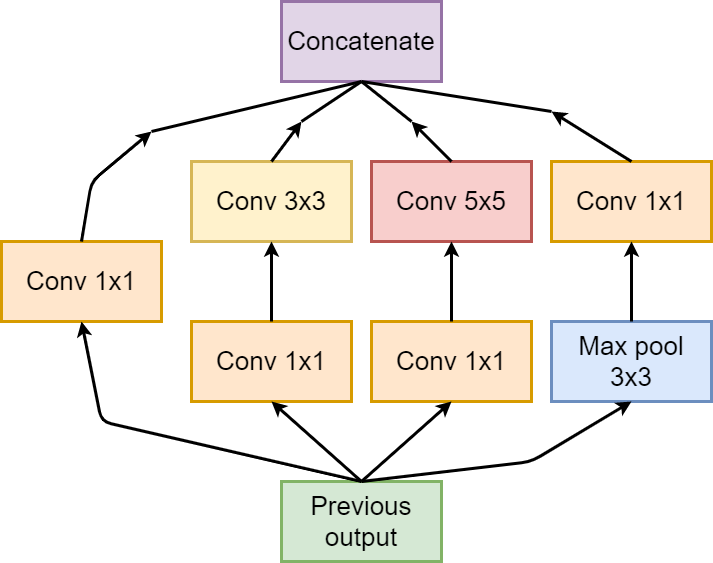
\includegraphics[width=2.5in]{images/inception_block.png}
	\caption{}
	\label{arch:inc}
\end{subfigure}%
\begin{subfigure}{0.5\textwidth}
	\centering
	\hspace{-1cm}
\includegraphics[width=3.5in]{images/resnet50.png}
	\caption{}
	\label{arch:res}
\end{subfigure}
\caption{(a) Diagram of a single inception block, adapted from \cite{Szegedy15}. "Conv 		1x1" represents a convolutional layer with kernel size $1\times1$ and "max pool 3x3" represents max pooling with pool size and stride of $3\times3$. The branching architecture with varying kernel sizes attempts to extract features of varying sizes from the input \cite{Szegedy15}. 
(b) The architecture of ResNet50, adapted from \cite{He15}. "Conv 1x1, N" is a convolutional layer with kernel size $1\times1$ and $N$ channels. All convolutional layers have stride of $1\times1$. The input to a skip connection block is put through three convolutional layers, and the output of this is concatenated with the original input. The factors next to each skip connection block represent a series of that number of blocks.}
\label{arch:arch}
\end{figure}

%\begin{figure}[!h]
%\centering
%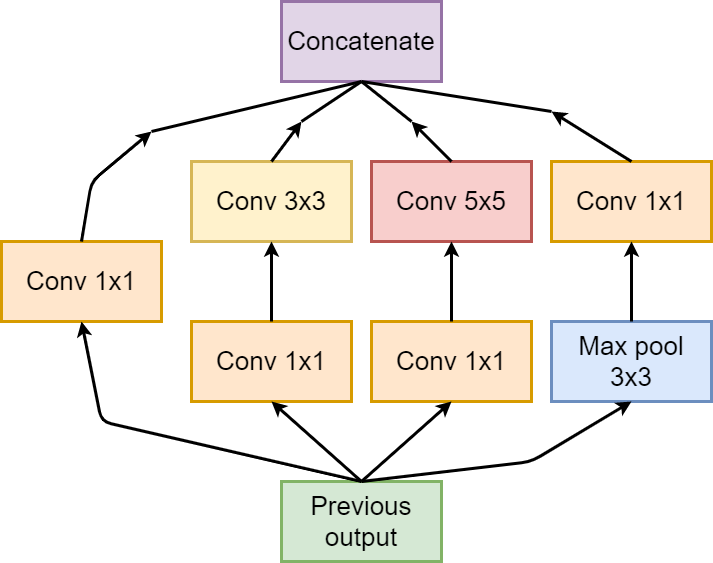
\includegraphics[width=4in]{images/inception_block.png}
%\caption{Diagram of a single inception block, adapted from \cite{Szegedy15}. "Conv 1x1" represents a convolutional layer with kernel size $1\times1$ and "max pool 3x3" represents max pooling with pool size and stride of $3\times3$. The branching architecture with varying kernel sizes attempts to extract features of varying sizes from the input.}
%\label{incblock}
%\end{figure}

%\begin{figure}[!h]
%\centering
%
\includegraphics[width=4.5in]{images/resnet50.png}
%\caption{The architecture of ResNet50, adapted from \cite{He15}. "Conv 1x1, N" is a convolutional layer with kernel size $1\times1$ and $N$ channels. All convolutional layers have stride of $1\times1$. The input to a skip connection block is put through three convolutional layers, and the output of this is concatenated with the original input. The factors next to each skip connection block represent a series of that many blocks.}
%\label{arch:res}
%\end{figure}

\subsection{Model training configurations}
We use the deep learning libraries TensorFlow and Keras to build and train all models \cite{Abadi16, Gulli17}. Model training is powered by NVIDIA CUDA, either on an NVIDIA RTX 2060 graphics card or cloud-based using Google Colaboratory \cite{Cook12, Bisong19}. All models use the categorical cross-entropy loss function and are updated with the Adam optimiser, detailed in the first semester report, with variable learning rate and other fixed hyperparameter settings of $\beta_1=0.9$, $\beta_2=0.999$, and $\epsilon=10^{-7}$ \cite{Heaton20, Kingma14}. Early stopping is applied to all models, with a patience of 30 epochs and based on validation set cost. The final saved model parameters correspond to the epoch of training with the lowest validation set cost. Based on investigations of the previous semester, random flipping in both the horizontal and vertical directions is applied to the minibatches of images throughout training \cite{Heaton20}. These are the only augmentations used. Model accuracy on a dataset is evaluated as the percentage of correctly classified images in the set. 

\subsection{Model tuning}
For each dataset, we train and tune Sequential, Inception and ResNet50 classifier models with the aim of maximising accuracy when evaluating on the test set. The hyperparameters we choose to vary include batch size and learning rate for all model types. For the Sequential models we also vary the number of convolutional layers and starting channels, and for the Inception models we vary the number Inception blocks and starting channels. The ResNet50 architecture is fixed. For every configuration tested we train the model ten times, recording the validation and test set accuracies at the end of each run. The model's parameters are reset between each run. The mean accuracies for the configuration are then calculated along with the standard deviations. Selection of hyperparameters is based on trial and error combined with grid-search methods. In a grid-search lists of values are specified for two or more hyperparameters, and models are trained with all possible combinations of the values \cite{Goodfellow16}.

\section{Classification tasks and results}
Here, the results for the models of each type achieving the highest mean test set accuracies for each phase classification task are presented. Architecture details are listed as number of convolutional layers, number of starting channels for Sequential models, and number of blocks, number of starting channels for Inception models. The error bars on the results summary graphs for each dataset represent the standard deviation of the test set accuracy. Model types are abbreviated as "Seq" for Sequential, "Inc" for Inception, and "RN50" for ResNet50. The y-axis scale is fixed at 50 to 100 percent to aid comparison of the results between each dataset.

The test set mean and standard deviation confusion matrices are given for the best model type and configuration in each case. Confusion matrix values represent the fraction of test set samples with a particular true label that the model assigned a particular predicted label. For the best performing model configurations, the confusion matrices are calculated for all ten individual trained models, and the mean and standard deviation are calculated for each value.

%Describe task
%Model specfifics
%Accuracy results
%Model comparisons
%Standard deviations
%Difference between validation and test
%Discussion of best con mat
%Interpretation

\subsection{Summary of first semester results}
The work of the first semester focussed on applying Sequential, Inception and ResNet models to three different LC phase classification tasks. These included a four-phase set with isotropic, nematic, cholesteric, and smectic, a binary set with smectic A and C, a general smectic set including fluid smectic, hexatic smectic, and soft crystal, and a six-phase smectic set including smectic A, C, I, F, and two soft crystal phases. The final models were trained three times each and the mean accuracy over all three runs calculated for the test sets. The error was calculated as half the range in accuracy. The results are summarised in Table \ref{sem1}.
\begin{table}[!htb]
\begin{center}
\caption{First semester mean test set percentage accuracies for final models and phase classification tasks.}
\begin{tabular}{l|c|c|c}
\toprule
\textbf{Dataset} & \textbf{No. of phases} & \textbf{Best model} & \textbf{Test accuracy/\%}\\
\midrule
Four-phase & 4 & Sequential 2 layers & $91\pm4$\\
Smectic A and C & 2 & Sequential 4 layers & $97\pm1$\\
General smectic & 3 & ResNet50 & $92\pm4$\\
Six-phase smectic & 6 & ResNet50 & $54\pm1$\\
\bottomrule
\omit
\label{sem1}
\end{tabular}
\end{center}
\end{table}
It was concluded that the poor performance in the more complex six-phase smectic task was a result of limited dataset size \cite{Heaton20}.

\subsection{Binary classifiers}
The binary classifiers predict which of two phases a LC texture is displaying. These serve as foundational investigations for model viability before attempting to build more complex multi-phase classifiers.

\subsubsection{ChSm}
Models in this first binary phase classification task attempt to differentiate between the cholesteric phase and all smectic phases in the complete dataset. The final results for the tuned models are displayed in Figure \ref{chsm:chsm} and the model configurations and accuracies are given in Table \ref{chsmtab}. All three model types achieve over 90\% mean test acuracy, with Inception the highest and ResNet50 the lowest. The extremely high capacity of ResNet50 could lead to some overfitting, despite usage of early stopping. Overall, the variances in accuracy suggest good stability in training the models, with no standard deviations greater than 3\%. The mean test accuracies are higher than validation in every case. However, the differences are small. This trend is most likely due to the relatively small size of the dataset, which could result in elevated sensitivity to the exact choice of videos to include in each set.
\begin{table}[!htb]
\begin{center}
\caption{Best results and corresponding model configuration details for the ChSm dataset. For the number of parameters, k represents multiples of one thousand and m represents one million.}
\begin{tabular}{l|c|c|c}
\toprule
\textbf{ChSm} & \textbf{Sequential} & \textbf{Inception} & \textbf{ResNet50}\\
\midrule
\textbf{Mean test accuracy/\%} & $96\pm3$ & $98\pm2$ & $93\pm3$\\
\textbf{Mean validation accuracy/\%} & $93\pm1$ & $95\pm2$ & $91\pm2$\\
\textbf{Architecture details} & 3, 64 & 1, 16 & N/A\\
\textbf{Batch size} & 16 & 16 & 16\\
\textbf{Learning rate} & $5\times10^{-5}$ & $1\times10^{-4}$ & $1\times10^{-4}$\\
\textbf{Trainable parameters} & 470 k & 497 k & 25.5 m\\
\bottomrule
\omit
\label{chsmtab}
\end{tabular}
\end{center}
\end{table} 
\begin{figure}[!h]
\centering
\begin{subfigure}{0.4\textwidth}
	\centering
	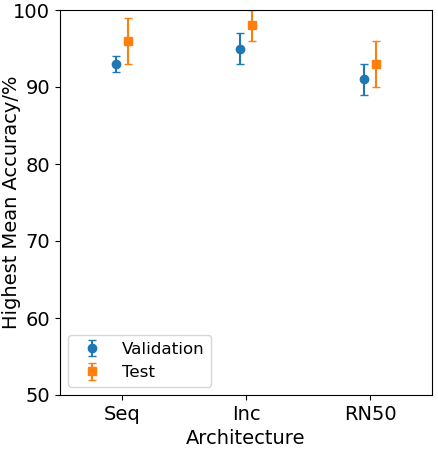
\includegraphics[width=2.5in]{images/Graphs/ChSm.png}
	\caption{}
	\label{chsm:graph}
\end{subfigure}%
\begin{subfigure}{0.25\textwidth}
	\centering
	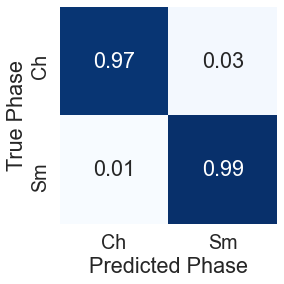
\includegraphics[width=1.5in]{images/ConMats/ChSm_mean.png}
	\caption{}
	\label{chsm:mean}
\end{subfigure}%
\begin{subfigure}{0.25\textwidth}
	\centering
	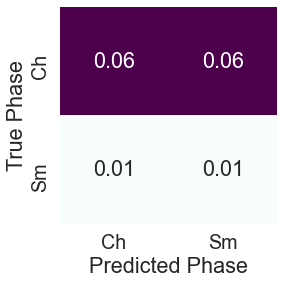
\includegraphics[width=1.5in]{images/ConMats/ChSm_std.png}
	\caption{}
	\label{chsm:std}
\end{subfigure}%
\caption{(a) Mean test and validation set accuracies for the best model of each type trained on the ChSm dataset. (b) Mean test set confusion matrix for the ChSm Inception model. (c) Standard deviations of test set confusion matrices for the ChSm Inception model.}
\label{chsm:chsm}
\end{figure}

The mean confusion matrix in Figure \ref{chsm:mean} for the Inception model shows that the inaccuracies in general stem from misidentifying the cholesteric phase as smectic, at 3\%. This is likely due to the large imbalance in the dataset in favour of the smectic class, which has approximately three times the number of samples. Such an imbalance may induce some bias in the model towards the larger class. In addition, the models are most unstable when processing cholesteric samples, as demonstrated by the standard deviation confusion matrix in Figure \ref{chsm:std}, with 6\% for both true cholesteric values. Again, this could be due to the class imbalance. There may also be some cholesteric images with features that are similar to some smectic ones. Overall, the ChSm task is successful in demonstrating that the CNN models can easily learn to distinguish between features of two broad and distinct LC phases.

\subsubsection{SmAC}
The fluid smectic A and C phases share similar textural features because the difference in order between the phases is subtle \cite{Dierking03}. One could, therefore, infer that the binary classification task on the SmAC dataset should be more challenging. The work of the previous semester implied that this is not the case, as the best model trained on a similar smectic A and C dataset achieved $97\pm1\%$ mean test set accuracy \cite{Heaton20}. We now attempt to verify and improve this result with the more robust method of performing ten training runs per model configuration as opposed to just three. The obtained results for the models tuned to the SmAC dataset are presented in Figure \ref{smac:smac} and Table \ref{smactab}. Both the Sequential and Inception models achieve an extremely high accuracy on the test set, with ResNet50 behind by 8\%. Again, the validation accuracies are lower for all models.
\begin{table}[!htb]
\begin{center}
\caption{Best results and corresponding model configuration details for the SmAC dataset.}
\begin{tabular}{l|c|c|c}
\toprule
\textbf{SmAC} & \textbf{Sequential} & \textbf{Inception} & \textbf{ResNet50}\\
\midrule
\textbf{Mean test accuracy/\%} & $99\pm1$ & $99\pm1$ & $91\pm2$\\
\textbf{Mean validation accuracy/\%} & $92\pm3$ & $95\pm3$ & $90\pm1$\\
\textbf{Architecture details} & 4, 8 & 2, 2 & N/A\\
\textbf{Batch size} & 16 & 16 & 16\\
\textbf{Learning rate} & $1\times10^{-4}$ & $1\times10^{-4}$ & $1\times10^{-5}$\\
\textbf{Trainable parameters} & 31 k & 34 k & 25.5 m\\
\bottomrule
\omit
\label{smactab}
\end{tabular}
\end{center}
\end{table}
\begin{figure}[!h]
\centering
\begin{subfigure}{0.4\textwidth}
	\centering
	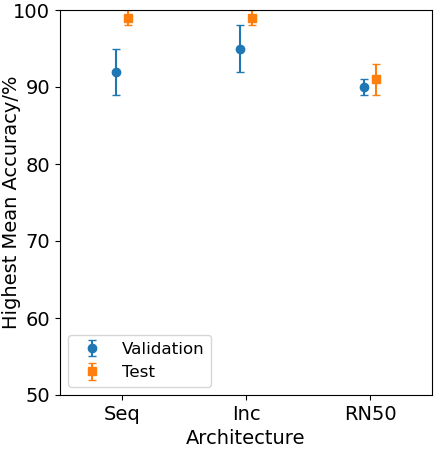
\includegraphics[width=2.5in]{images/Graphs/SmAC.png}
	\caption{}
	\label{smac:graph}
\end{subfigure}%
\begin{subfigure}{0.25\textwidth}
	\centering
	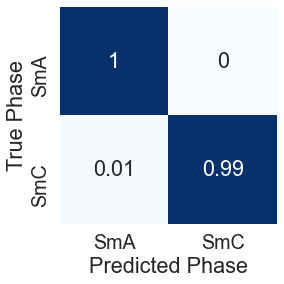
\includegraphics[width=1.5in]{images/ConMats/SmAC_mean.png}
	\caption{}
	\label{smac:mean}
\end{subfigure}%
\begin{subfigure}{0.25\textwidth}
	\centering
	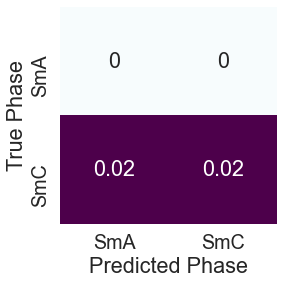
\includegraphics[width=1.5in]{images/ConMats/SmAC_std.png}
	\caption{}
	\label{smac:std}
\end{subfigure}%
\caption{(a) Mean test and validation set accuracies for the best model of each type trained on the SmAC dataset. (b) Mean test set confusion matrix for the SmAC Inception model. (c) Standard deviations of test set confusion matrices for the SmAC Inception model.}
\label{smac:smac}
\end{figure}

The mean confusion matrix for the Inception model in Figure \ref{smac:mean} shows that on all ten training runs, the model is 100\% accurate in identifying the smectic A phase in the test set. The only confusion is an average rate of 1\% misidentification of smectic C as A, despite the slight imbalance of the dataset with almost two times more smectic C samples than A. The results of the first semester for smectic A and C have been reinforced and improved upon, demonstrating the suitability of CNNs in cases with fine differences between image features. 

\subsubsection{SmIF}
The hexatic smectic I and F binary classification task is another one in which the phases display similar features due to similar underlying structure \cite{Dierking03}. The results and model configurations for the SmIF dataset are displayed in Figure \ref{smif:smif} and Table \ref{smiftab}. Overall model performance is worse than for the previous datasets, with the highest mean test set accuracy coming from the Sequential architecture, at $93\pm6\%$. In addition, there are large variances in accuracy for SmIF. This could be a result of the relatively small size of the dataset, which could cause instability in training the models as there are not enough samples to consistently learn the correct characteristic features for each phase. The poorer performance and high variance could also suggest that the features distinguishing smectic I and F are more subtle than in, for example, the case of smectic A and C. The performance of ResNet50 is particularly low. This is in part because the training time is longer than for the sequential and inception models, which allows for fewer tuning attempts. 
\begin{table}[!htb]
\begin{center}
\caption{Best results and corresponding model configuration details for the SmIF dataset.}
\begin{tabular}{l|c|c|c}
\toprule
\textbf{SmIF} & \textbf{Sequential} & \textbf{Inception} & \textbf{ResNet50}\\
\midrule
\textbf{Mean test accuracy/\%} & $93\pm6$ & $82\pm14$ & $66\pm12$\\
\textbf{Mean validation accuracy/\%} & $84\pm12$ & $88\pm12$ & $68\pm8$\\
\textbf{Architecture details} & 3, 128 & 2, 8 & N/A\\
\textbf{Batch size} & 16 & 16 & 16\\
\textbf{Learning rate} & $1\times10^{-4}$ & $1\times10^{-4}$ & $1\times10^{-5}$\\
\textbf{Trainable parameters} & 1.9 m & 538 k & 25.5 m\\
\bottomrule
\omit
\label{smiftab}
\end{tabular}
\end{center}
\end{table}
\begin{figure}[!h]
\centering
\begin{subfigure}{0.4\textwidth}
	\centering
	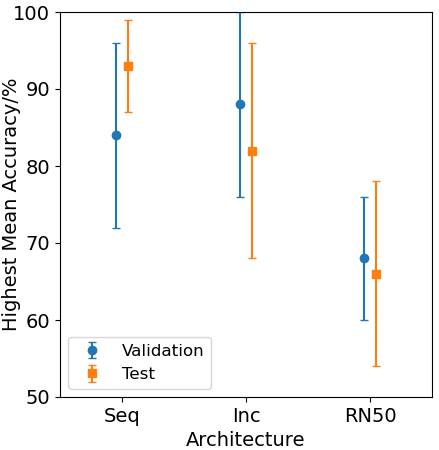
\includegraphics[width=2.5in]{images/Graphs/SmIF.png}
	\caption{}
	\label{smif:graph}
\end{subfigure}%
\begin{subfigure}{0.25\textwidth}
	\centering
	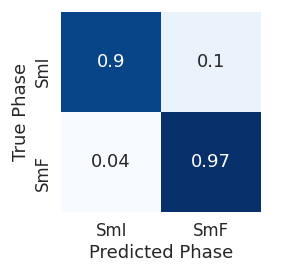
\includegraphics[width=1.7in]{images/ConMats/SmIF_mean.png}
	\caption{}
	\label{smif:mean}
\end{subfigure}%
\begin{subfigure}{0.25\textwidth}
	\centering
	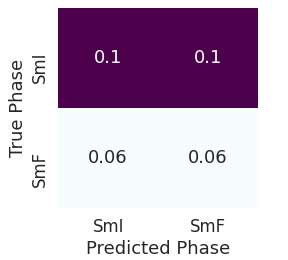
\includegraphics[width=1.7in]{images/ConMats/SmIF_std.png}
	\caption{}
	\label{smif:std}
\end{subfigure}%
\caption{(a) Mean test and validation set accuracies for the best model of each type trained on the SmIF dataset. (b) Mean test set confusion matrix for the SmIF Sequential model. (c) Standard deviations of test set confusion matrices for the SmIF Sequential model.}
\label{smif:smif}
\end{figure}

Figure \ref{smif:mean} shows the mean test set confusion matrix for the SmIF Sequential model. From this we see the greatest source of inaccuracy is in the true smectic I sample predictions, with 90\% mean test accuracy as opposed to 97\% for smectic F. The two classes are well balanced in this case, which provides no explanation for the inaccuracy. It may instead perhaps stem from images in the dataset that have been taken near the point of a phase transition between smectic I and F, which could result in some overlap of important features from each phase in the image. Therefore, the model could be exhibiting a bias towards smectic F if its confidence identifying smectic F features is greater than for smectic I. The standard deviation confusion matrix in Figure \ref{smif:std} shows that true phase smectic I accuracy is also more unstable than smectic F, which provides further evidence that the model is less confident in extracting the features of smectic I.

The performance on the SmIF dataset is satisfactory in that the models perform substantially better than randomly guessing. However, there is room for improvement. This may only be facilitated by expansion of the dataset with more videos from smectic I and F phases, which would provide more samples for the models to learn a more accurate interpretation of the subtle textural features.

\subsection{Multi-phase classifiers}
Having demonstrated success in binary LC phase classification, we now move on to the wider tasks of classification of more than two phases at a time.

\subsubsection{ChSm2}
The ChSm2 dataset contains all phases in the complete dataset, with smectic A and C grouped into the fluid smectic class and smectic I and F grouped into the hextic smectic class. The hexatic smectic class contains more images than the entire SmIF dataset because images from one video displaying the hexatic smectic phase could not be further labelled as smectic I or F. Figure \ref{chsm2:chsm2} and Table \ref{chsm2tab} give the results and model configurations for this dataset. We see similar performance from the Sequential and Inception models, with both reaching 85\% mean test accuracy. ResNet50 falls behind again on this task, most likely for similar reasons of overfitting and fewer attempts at tuning as before. With no standard deviations greater than 3\%, model training and accuracy is relatively stable for the ChSm2 task. Overall performance is low in comparison to the binary datasets, which could be explained by the increased complexity and size of the task with a greater number of phases and, subsequently, more features to learn.
\begin{table}[!htb]
\begin{center}
\caption{Best results and corresponding model details for the ChSm2 dataset.}
\begin{tabular}{l|c|c|c}
\toprule
\textbf{ChSm2} & \textbf{Sequential} & \textbf{Inception} & \textbf{ResNet50}\\
\midrule
\textbf{Mean test accuracy/\%} & $85\pm2$ & $85\pm3$ & $72\pm2$\\
\textbf{Mean validation accuracy/\%} & $82\pm2$ & $83\pm3$ & $67\pm3$\\
\textbf{Architecture details} & 3, 64 & 1, 8 & N/A\\
\textbf{Batch size} & 16 & 16 & 16\\
\textbf{Learning rate} & $5\times10^{-5}$ & $1\times10^{-4}$ & $1\times10^{-4}$\\
\textbf{Trainable parameters} & 470 k & 125 k & 25.5 m\\
\bottomrule
\omit
\label{chsm2tab}
\end{tabular}
\end{center}
\end{table}
\begin{figure}[!h]
\centering
\begin{subfigure}{0.37\textwidth}
	\centering
	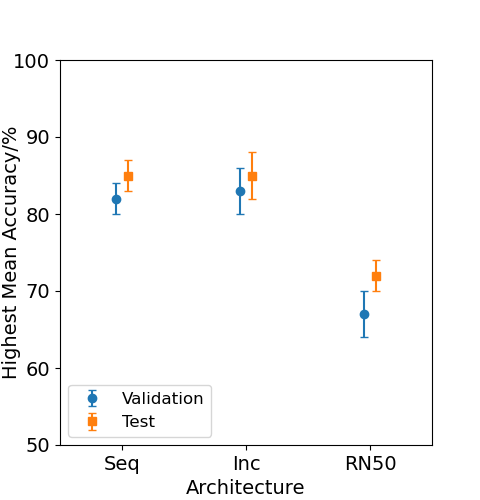
\includegraphics[width=2.5in]{images/Graphs/ChSm2.png}
	\caption{}
	\label{chsm2:graph}
\end{subfigure}%
\begin{subfigure}{0.3\textwidth}
	\centering
	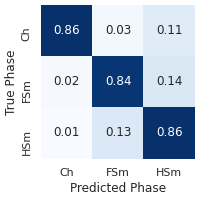
\includegraphics[width=2in]{images/ConMats/ChSm2_mean.png}
	\caption{}
	\label{chsm2:mean}
\end{subfigure}%
\begin{subfigure}{0.3\textwidth}
	\centering
	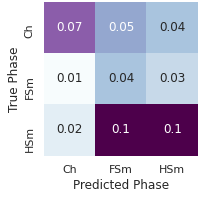
\includegraphics[width=2in]{images/ConMats/ChSm2_std.png}
	\caption{}
	\label{chsm2:std}
\end{subfigure}%
\caption{(a) Mean test and validation set accuracies for the best model of each type trained on the ChSm2 dataset. (b) Mean test set confusion matrix for the ChSm2 Sequential model. (c) Standard deviations of test set confusion matrices for the ChSm2 Sequential model.}
\label{chsm2:chsm2}
\end{figure}

Displayed in Figure \ref{chsm2:mean} is the mean test set confusion matrix for the Sequential model. Surprisingly, the true cholesteric samples are most often mislabelled as hexatic smectic, at 11\%. This is counter-intuitive because the hextic smectic phase has higher order than fluid smetic, which would normally result in greater similarity between the cholesteric and fluid smectic phases rather than between cholesteric and hexatic smectic. There is also generally high confusion between the fluid and hexatic smectic phases, and relatively high instability in accuracy for true hexatic smectic samples, when studying Figure \ref{chsm2:std}. These results could be explained by the similarity of texture features over all fluid and hexatic smectic phases, with more data and perhaps more rigorous tuning required to push accuracy further.

\subsubsection{ChSm4}
The final dataset, ChSm4, contains five classes with all individual phases of the complete dataset. This is the most ambitious and challenging of all the phase classification tasks, requiring the models to learn numerous subtle features to distinguish between a closely related series of LC phases. The results from extensive tuning are presented in Figure \ref{chsm4:chsm4} and Table \ref{chsm4tab}. We again see good performance on the test set from the Sequential and Inception models, at 87\% and 86\% mean accuracy respectively, with ResNet50 performing worse by approximately 20\%. Of note is the particularly poor mean validation accuracy for all model types, with none reaching 70\%. This is again indicative that the final result is sensitive to the specific choice of videos placed in each sub-dataset, likely due to the small overall size of the complete dataset. 
\begin{table}[!h]
\begin{center}
\caption{Best results and corresponding model configuration details for the ChSm4 dataset.}
\begin{tabular}{l|c|c|c}
\toprule
\textbf{ChSm4} & \textbf{Sequential} & \textbf{Inception} & \textbf{ResNet50}\\
\midrule
\textbf{Mean test accuracy/\%} & $87\pm3$ & $86\pm4$ & $66\pm7$\\
\textbf{Mean validation accuracy/\%} & $65\pm2$ & $68\pm5$ & $60\pm5$\\
\textbf{Architecture details} & 3, 128 & 2, 4 & N/A\\
\textbf{Batch size} & 16 & 16 & 16\\
\textbf{Learning rate} & $1\times10^{-5}$ & $1\times10^{-4}$ & $5\times10^{-4}$\\
\textbf{Trainable parameters} & 1.9 m & 135 k & 25.5 m\\
\bottomrule
\omit
\label{chsm4tab}
\end{tabular}
\end{center}
\end{table}
\begin{figure}[!h]
\centering
\begin{subfigure}{0.4\textwidth}
	\centering
	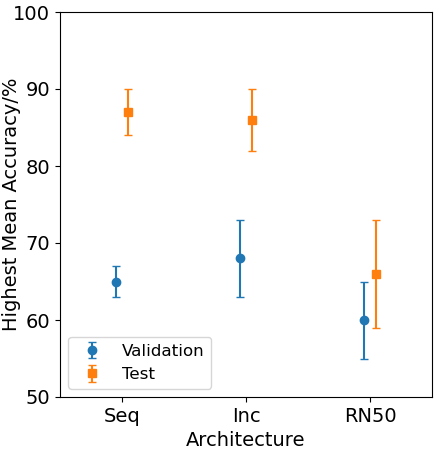
\includegraphics[width=2.5in]{images/Graphs/ChSm4.png}
	\caption{}
	\label{chsm4:graph}
\end{subfigure}

\begin{subfigure}{0.4\textwidth}
	\centering
	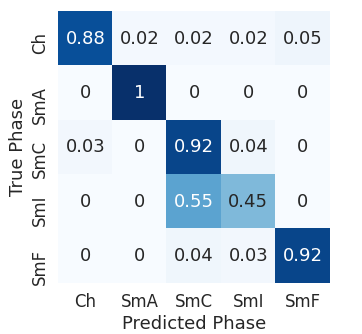
\includegraphics[width=2.5in]{images/ConMats/ChSm4_mean.png}
	\caption{}
	\label{chsm4:mean}
\end{subfigure}%
\begin{subfigure}{0.4\textwidth}
	\centering
	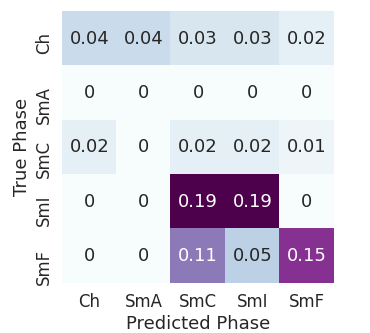
\includegraphics[width=2.5in]{images/ConMats/ChSm4_std.png}
	\caption{}
	\label{chsm4:std}
\end{subfigure}%
\caption{(a) Mean test and validation set accuracies for the best model of each type trained on the ChSm4 dataset. (b) Mean test set confusion matrix for the ChSm4 Sequential model. (c) Standard deviations of test set confusion matrices for the ChSm4 Sequential model.}
\label{chsm4:chsm4}
\end{figure}

Upon constructing the mean test set confusion matrix for the Sequential model, in Figure \ref{chsm4:mean}, the main source of inaccuracy is revealed. The true smectic I samples are mislabelled as smectic C 55\% of the time on average, with a large standard deviation of 19\% as seen in Figure \ref{chsm4:std}. This suggests that there may be overlap in the model's learned features between the smectic C and I phases. The model is largely successful in identifying all other phases, each correctly predicted approximately 90\% of the time with smectic A correct 100\% of the time. The accuracy on true smectic F samples has a high standard deviation of 15\%, similarly to smectic I. These results combined provide insight into the inaccuracies of the ChSm2 task, which likely also suffers from confusion between smectic C and I samples.

The success of the models applied to the ChSm4 dataset is notable. However, training on a vastly expanded dataset would perhaps allow model accuracy and stability to be improved. This would require longer training times because larger model capacities would be required to extract more meaningful features from the data. A more balanced dataset with better representation for the smectic A, I and F phases may also be beneficial.

\section{Conclusions}
%summarise results
%comparison previous semester
%discuss best/worst model types
%limitations
%dataset size
%further research
In this second half of the project, we have expanded the overall dataset and trained and tuned models to a high average test set accuracy in a greater number of ambitious LC phase classification tasks. A summary of the best results for each phase grouping is presented in Table \ref{sem2}.
\begin{table}[!htb]
\begin{center}
\caption{Results for the best tuned model for each prepared dataset.}
\begin{tabular}{l|c|c|c}
\toprule
\textbf{Dataset} & \textbf{No. of phases} & \textbf{Best model type} & \textbf{Mean test accuracy/\%}\\
\midrule
ChSm & 2 & Inception & $98\pm2$\\
SmAC & 2 & Inception & $99\pm1$\\
SmIF & 2 & Sequential & $93\pm6$\\
ChSm2 & 3 & Sequential & $85\pm2$\\
ChSm4 & 5 & Sequential & $87\pm3$\\
\bottomrule
\omit
\label{sem2}
\end{tabular}
\end{center}
\end{table}
The results of the previous semester have been expanded, improved, and consolidated, further demonstrating the potential of CNN models in the automatic identification of LC phase textures. Of particular note is the improvement in model performance in tasks involving the hexatic smectic phases, which were relatively unsuccessful in the first half of the project \cite{Heaton20}. This has been achieved through the addition of more smectic I and F texture images to the dataset as well as more robust model training and tuning methodology. The current literature has been further expanded upon, which remains limited to classification of simulated textures of non-smectic LC phases \cite{Sigaki20}. 

Overall the Sequential models have proved most successful, achieving the highest mean test accuracies in the three most complex classification tasks. The inception models follow closely behind with comparable results in all cases. Contradictory to the results of the previous semester, ResNet50 has performed the worst on all datasets. However, it did produce mean test accuracies above 90\% on the ChSm and SmAC datasets. The generally poor performance suggests the capacity of the model is too high and overfitting to the training set has occurred. Furthermore, the size of ResNet50 results in training times much longer than for the other models. For this reason, fewer hyperparameter tuning cycles have been performed.

Throughout the project, dataset size has been the key limitation. For certain classification tasks, particularly those involving the smectic I and F phases, the results could potentially be improved by further balancing and expanding the dataset with more samples. Confusion between smetic C and I, as in the case of the ChSm4 results, is a limitation that could be investigated further. Texture similarity between the phases is a likely cause of the inaccuracy, which could again be tested further by incorporation of samples from different LC compounds. Including PM videos from an extended range of compounds would be beneficial in allowing the models to learn more general textural features from each phase, improving accuracy when applied to new unseen samples. In addition, the limited dataset size has resulted in model accuracy being sensitive to the specific choice of training, validation and test set split. This is seen in the discrepancies between validation and test accuracy in some tasks, especially so for ChSm4.

As an outlook to future potential work, an ambitious goal would be to establish a vastly expanded dataset spanning more phases, such as soft crystal. Larger models such as ResNet50 would be necessary to obtain high accuracies on such a more complex classification task. Alternatives to CNNs could be investigated, such as the promising Transformer network architectures which have seen success in computer vision tasks involving extremely large datasets \cite{Khan2021TransformersIV}.

\bibliography{report2}

\appendix
\appendixpage
\section{Data distributions} \label{datdist}
The exact numbers of images of each phase in each sub dataset are presented here.
\begin{table}[!htb]
\begin{center}
\caption{Image count and distribution for each LC phase class.}
\begin{tabular}{l|c|c|c|c|c|c|c|c}
\toprule
\textbf{Phase} & \textbf{Ch} & \textbf{Sm} & \textbf{FSm} & \textbf{HSm} & \textbf{SmA} & \textbf{SmC} & \textbf{SmI} & \textbf{SmF}\\
\midrule
\textbf{Training} & 1148 & 3598 & 2110 & 1488 & 722 & 1388 & 918 & 570\\
\textbf{Validation} & 245 & 853 & 481 & 372 & 180 & 301 & 198 & 168\\
\textbf{Test} & 253 & 881 & 515 & 366 & 204 & 311 & 210 & 162\\
\textbf{Totals} & 1646 & 5332 & 3106 & 2226 & 1106 & 2000 & 1326 & 900\\
\bottomrule
\omit
\label{chsmdist}
\end{tabular}
\end{center}
\end{table}

\begin{comment}
\begin{table}[!htb]
\begin{center}
\caption{Image count and distribution for the ChSm dataset.}
\begin{tabular}{l|c|c|c}
\toprule
\textbf{ChSm} & \textbf{Ch} & \textbf{Sm} & \textbf{Totals}\\
\midrule
\textbf{Training} & 1148 & 3598 & 4746\\
\textbf{Validation} & 245 & 853 & 1098\\
\textbf{Test} & 253 & 881 & 1134\\
\textbf{Totals} & 1646 & 5332 & 6978\\
\bottomrule
\omit
\label{chsmdist}
\end{tabular}
\end{center}
\end{table}
\begin{table}[!htb]
\begin{center}
\caption{Image count and distribution for the SmAC dataset.}
\begin{tabular}{l|c|c|c}
\toprule
\textbf{SmAC} & \textbf{SmA} & \textbf{SmC} & \textbf{Totals}\\
\midrule
\textbf{Training} & 722 & 1388 & 2110\\
\textbf{Validation} & 180 & 301 & 481\\
\textbf{Test} & 204 & 311 & 515\\
\textbf{Totals} & 1106 & 2000 & 3106\\
\bottomrule
\omit
\label{smacdist}
\end{tabular}
\end{center}
\end{table}
\begin{table}[!htb]
\begin{center}
\caption{Image count and distribution for the SmIF dataset.}
\begin{tabular}{l|c|c|c}
\toprule
\textbf{SmIF} & \textbf{SmI} & \textbf{SmF} & \textbf{Totals}\\
\midrule
\textbf{Training} & 918 & 570 & 1488\\
\textbf{Validation} & 198 & 168 & 366\\
\textbf{Test} & 210 & 162 & 372\\
\textbf{Totals} & 1326 & 900 & 2226\\
\bottomrule
\omit
\label{smifdist}
\end{tabular}
\end{center}
\end{table}
\begin{table}[!htb]
\begin{center}
\caption{Image count and distribution for the ChSm2 dataset.}
\begin{tabular}{l|c|c|c|c}
\toprule
\textbf{ChSm2} & \textbf{Ch} & \textbf{FSm} & \textbf{HSm} & \textbf{Totals}\\
\midrule
\textbf{Training} & 1148 & 2110 & 1488 & 4746\\
\textbf{Validation} & 245 & 481 & 372 & 1098\\
\textbf{Test} & 253 & 515 & 366 & 1134\\
\textbf{Totals} & 1646 & 3106 & 2226 & 6978\\
\bottomrule
\omit
\label{chsm2dist}
\end{tabular}
\end{center}
\end{table}
\begin{table}[!htb]
\begin{center}
\caption{Image count and distribution for the ChSm4 dataset.}
\begin{tabular}{|l|c|c|c|c|c|c|}
\toprule
\textbf{ChSm4} & \textbf{Ch} & \textbf{SmA} & \textbf{SmC} & \textbf{SmI} & \textbf{SmF} &\textbf{Totals}\\
\midrule
\textbf{Training} & 1148 & 722 & 1388 & 534 & 420 & 4212\\
\textbf{Validation} & 245 & 180 & 301 & 108 & 90 & 924\\
\textbf{Test} & 253 & 204 & 311 & 120 & 120 & 1008\\
\textbf{Total} & 1646 & 1106 & 2000 & 762 & 630 & 6144\\
\bottomrule
\omit
\label{chsm4dist}
\end{tabular}
\end{center}
\end{table}
\end{comment}

\end{document}